% !TEX program = pdflatex
\documentclass{article}
\usepackage{tikz}
\usetikzlibrary{calc}

\begin{document}
\section*{Setting the centre punch}
\begin{figure}[ht]\centering
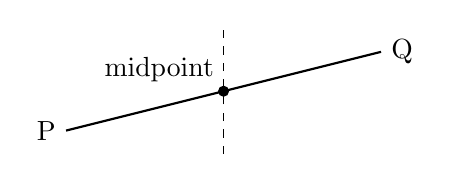
\begin{tikzpicture}

\coordinate (P) at (0,0);\coordinate (Q) at (4,1);
\coordinate (M) at ($(P)!.5!(Q)$);
\draw[thick] (P) node[left] {P}--(Q) node[right] {Q};
\draw[dashed] ($(M)+(0,-.8)$)--($(M)+(0,.8)$);
\fill (M) circle (2pt) node[above left] {midpoint};
\end{tikzpicture}\caption{The centre line passes through the half-distance mark.}\end{figure}
\end{document}
